\documentclass[12pt,a4paper]{article}
\usepackage[utf8]{inputenc}
\usepackage[T1]{fontenc}
\usepackage{amsmath,amssymb,amsfonts,mathtools}
\usepackage{amsthm}
\usepackage{geometry}
\geometry{left=2cm,right=2cm,top=2cm,bottom=2cm}
\usepackage{booktabs}
\usepackage{tabularx}
\usepackage{hyperref}
\usepackage{url}
\usepackage{xcolor}
\usepackage{titlesec}
\usepackage{microtype}
\usepackage{enumitem}
\usepackage{tikz}
\usepackage{pgfplots}
\pgfplotsset{compat=1.18}


\newtheorem{axiom}{Axiom}
\newtheorem{remark}{Bemerkung}
\newtheorem{theorem}{Theorem}[section]
\DeclareMathOperator*{\Tr}{Tr}

\hypersetup{
	colorlinks=true,
	linkcolor=blue,
	citecolor=blue,
	urlcolor=blue,
}

\titleformat{\section}{\Large\bfseries}{\thesection}{1em}{}
\titleformat{\subsection}{\large\bfseries}{\thesubsection}{1em}{}

\begin{document}
	
	\begin{titlepage}
		\centering
		\vspace*{1cm}
		
		{\Huge\bfseries \(K_{\mathrm{eff}} > 1\) als ontologisches Erstprinzip\par}
		\vspace{0.3cm}
		{\Large\bfseries Der universelle Skalierungsexponent \(\beta = 2/3\), die elektroschwache Skala\par}
		\vspace{0.1cm}
		{\Large\bfseries und die Quantisierung der Fermionenmassen\par}
		\vspace{0.5cm}
		{\large Eine transparente Synthese aus Axiomen, empirischen Belegen und Phänomenologie\par}
		
		\vspace{1cm}
		
		{\large Alexey V. Yakushev\par}
		\vspace{0.3cm}
		{\normalsize Yakushev Research, \url{https://yuct.org/}\par}
		
		\vspace{0.5cm}
		{\sffamily\footnotesize \textbf DOI: \url{https://doi.org/10.5281/zenodo.18444598}}%
		
		\vspace{1.0cm}
		
		{\normalsize Version 6.3 (mit Neutrinomassen-Hypothese), April 2026\par}
		\vspace{0.3cm}
		{\normalsize DOI: \texttt{10.5281/zenodo.18444598}\par}
		
		\vfill
		
		\begin{abstract}
			\noindent
			Wir präsentieren die definitive logische Struktur der Yakushev Unified Coordination Theory (YUCT).  Jede Aussage ist entweder ein \textbf{Axiom} (irreduzibles Postulat), ein \textbf{Theorem} (aus den Axiomen bewiesen), ein \textbf{empirisches Gesetz} (robust beobachtet) oder eine \textbf{phänomenologische Anpassung} (eingeschränkt, aber noch nicht abgeleitet).  Aus der Definition der Koordinationseffizienz \(K_{\mathrm{eff}} > 1\) und drei strukturellen Axiomen beweisen wir, dass der Redundanzfaktor des Wörterbuchs \(q = 2/3\) beträgt.  Der universelle Exponent \(\beta = 2/3\) ist ein \textbf{empirisches Gesetz}, das durch mehr als ein Dutzend unabhängiger Experimente auf atomarer, biologischer, geophysikalischer und kosmologischer Skala bestätigt wurde.  Aus \(\beta = 2/3\) leiten wir die algebraischen Konstanten \(S_{\mathrm{odd}} = 1.2\) und \(S_{\mathrm{even}} = 0.8\) (geschlossene algebraische Schleife) ab.  Unter Verwendung der Anzahl der Weyl-Fermionenfreiheitsgrade (\(96\)) erhalten wir die elektroschwache Skala (\(m_W \approx 80.4\) GeV) bis auf einen einzigen Faktor \(\xi_W\).  Dieselbe algebraische Struktur liefert ein Skalierungsquant \(q = (3/2)^{1/3}\).  Die Massen der neun geladenen Fermionen liegen auf einer halbzahligen Leiter mit einer Genauigkeit von besser als \(1\%\) (die spezifischen Quantenzahlen \(N_f\) sind derzeit angepasst).  Die diskrete Struktur dieser Leiter ist eine \textbf{falsifizierbare Vorhersage}: Jedes zukünftige Teilchen mit einer Masse außerhalb der erlaubten Menge \(\{m_e q^{N/2}\}\) würde die Theorie widerlegen.  Für das leichteste Neutrino sind die erlaubten Massen \(\{0.0234, 0.0268, 0.0307, 0.0352, \dots\}\) eV.  Die Theorie enthält keine einstellbaren kontinuierlichen Parameter und macht mehrere weitere konkrete, überprüfbare Vorhersagen.
			
			Darüber hinaus stellen wir eine Variationshypothese vor, die die spezifische Neutrinoquantenzahl \(N_{\nu} = -125\) (Masse \(\approx 0.023\) eV) durch Maximierung der gesamten Koordinationsleistung des Fermionensektors auswählt.  Diese Vorhersage ist falsifizierbar und würde, falls bestätigt, die Theorie stärken.
		\end{abstract}
		
		\vspace{1cm}
		\textcopyright\ 2026 Alexey V. Yakushev. Alle Rechte vorbehalten.
	\end{titlepage}
	
	\tableofcontents
	\newpage
	
	\section{Einleitung: Koordination versus Information}
	\label{sec:intro}
	
	Shannons Theorie der Kommunikation begrenzt die Rate, mit der Information durch einen Kanal übertragen werden kann.  Dennoch ist die Natur voller Prozesse, bei denen ein kurzes Signal eine Reaktion auslöst, deren Informationsgehalt den des Signals bei weitem übersteigt: Ein Pheromonmolekül löst komplexes Verhalten aus, ein Startcodon initiiert die Proteinsynthese, ein kurzer Befehl aktiviert eine geplante Operation.  Die zusätzliche Information wird nicht in Echtzeit übertragen; sie ist bereits in einem \textbf{Wörterbuch} gespeichert, das während einer Offline-Phase verteilt wurde.
	
	Das Yakushev-Protokoll für synchrone verteilte Koordination (YPSDC) formalisiert diesen universellen Mechanismus:
	\begin{enumerate}[label=(\roman*)]
		\item \textbf{Offline-Phase:} Ein Wörterbuch \(\mathcal{D}\) mit \(M\) möglichen Aktionen (Zuständen, Nachrichten) wird unter den Agenten geteilt.  Jede Aktion \(A_i\) benötigt \(n_i\) Bits zur vollständigen Beschreibung.
		\item \textbf{Online-Phase:} Um die Aktion \(A_k\) zu aktivieren, wird nur ihr Index \(\kappa_k\) übertragen.  Bei gleichwahrscheinlichen Indizes beträgt die Indexlänge \(\ell = \log_2 M\) Bits.
	\end{enumerate}
	Die \textbf{Koordinationseffizienz} ist definiert als
	\begin{equation}
		\boxed{K_{\mathrm{eff}} = \frac{H(\mathcal{A})}{H(\kappa)} = \frac{\text{Aktionsentropie}}{\text{Indexentropie}} \ge 1},
		\label{eq:keff-def}
	\end{equation}
	wobei \(H\) die Shannon-Entropie bezeichnet.  Kein physikalisches Gesetz wird verletzt: Der Index wird mit \(v \le c\) übertragen; die zusätzliche Information wird lokal aus dem bereits vorhandenen Wörterbuch bezogen.
	
	\begin{center}
		\fbox{%
			\begin{minipage}{0.9\textwidth}
				\textbf{Ontologisches Prinzip:} \(K_{\mathrm{eff}} > 1\) ist eine notwendige Bedingung dafür, dass ein komplexes System seine Identität über die Zeit hinweg bewahren kann.  Ein System mit \(K_{\mathrm{eff}} = 1\) würde stets hinter seiner Umgebung zurückbleiben und zerstört werden.  Daher muss die Realität selbst als ein Koordinationsnetzwerk strukturiert sein.
			\end{minipage}%
		}
	\end{center}
	
	\section{Axiome hierarchischer Koordinationsnetzwerke}
	
	Ein Koordinationsnetzwerk besteht aus geschachtelten Clustern.
	
	\begin{axiom}[Hierarchische Skaleninvarianz] \label{ax:A1}
		Ein Cluster der Stufe \(n\) hat die lineare Größe \(L_n\) mit \(L_{n+1} = \lambda L_n\) (\(\lambda > 1\)).  Die Anzahl der Agenten skaliert wie \(N(L) \propto L^{d_f}\), wobei \(d_f\) die fraktale Dimension ist.  Für \(n \to \infty\) strebt das Verhältnis \(K_{\mathrm{eff},n+1}/K_{\mathrm{eff},n}\) gegen eine Konstante, was eine Potenzgesetz-Hierarchie impliziert.
	\end{axiom}
	
	\begin{theorem}[Minimale Wörterbuchentropie]
		\label{thm:minimal-dict}
		Das minimale Koordinationswörterbuch, das zuverlässig eine binäre Alternative unterscheiden kann, besitzt eine gesamte Shannon-Entropie von exakt \(2\) Bits (in Einheiten von \(k_B\ln 2\)).  Folglich erfüllt das vollständige hierarchische Wörterbuch \(S_{\mathrm{odd}} + S_{\mathrm{even}} = 2\).
	\end{theorem}
	
	\begin{proof}
		Ein minimales Wörterbuch muss nur eine einzige Ja/Nein-Frage beantworten: „Ist die Aktion \(A\) eingetreten?‟  Es enthält daher zwei Einträge, \(\mathcal{A} = \{A_0, A_1\}\), mit gleicher A-priori-Wahrscheinlichkeit, also
		\[
		H(\mathcal{A}) = \log_2 2 = 1\ \text{Bit}.
		\]
		Um einen der beiden Einträge zu aktivieren, wird ein Index \(\kappa \in \{0,1\}\) der Länge \(\ell = \log_2 2 = 1\)~Bit übertragen, woraus \(H(\mathcal{K}) = 1\)~Bit folgt.
		
		Der Empfänger muss sich jedoch auch sicher sein, dass der Index die beabsichtigte Aktion korrekt identifiziert; andernfalls würde ein einzelner Bitfehler die Koordination zerstören.  Diese Sicherheit erfordert ein zusätzliches Verifikationsbit, das im Wörterbuch gespeichert ist.  Daher beträgt die gesamte Wörterbuchentropie
		\[
		S_{\min} = H(\mathcal{A}) + H(\text{Verifikation}) = 1 + 1 = 2\ \text{Bits}.
		\]
		In der unendlichen Hierarchie (Abschnitt~\ref{sec:algebraic-loop}) wird diese minimale Struktur durch die Summen \(S_{\mathrm{odd}} + S_{\mathrm{even}} = 2\) realisiert, was die absolute Skala ohne jeden einstellbaren Parameter festlegt.
	\end{proof}
	
	\begin{axiom}[Einbettung in drei Dimensionen] \label{ax:A3}
		Die Agenten befinden sich in einem Raum der Dimension \(D = 3\).  Die Koordinationszeit für einen Cluster der Größe \(L\) beträgt \(\tau(L) = L/c\) und ist durch die Lichtgeschwindigkeit begrenzt.
	\end{axiom}
	
	
	\section{Theorem: Der Redundanzfaktor \(q = 2/3\)}
	
	Die Entropie des Wörterbuchs auf der tiefsten Stufe sei \(H_1\).  Nach Axiom \ref{ax:A1} skalieren die Entropien aufeinanderfolgender Stufen geometrisch: \(H_{l+1} = q H_l\) mit \(0 < q < 1\).  Die Gesamtentropie der unendlichen Hierarchie beträgt
	\[
	\sum_{l=1}^{\infty} H_l = \frac{H_1}{1-q}.
	\]
	Axiom \ref{ax:A2} verlangt, dass diese Summe gleich \(2\) ist.  Wir postulieren ferner, dass \(H_1 = q\) (die erste Stufe trägt die Information eines Redundanzfaktors; dies ist die einfachste selbstkonsistente Wahl).  Dann gilt
	\begin{equation}
		\frac{q}{1-q} = 2 \quad\Longrightarrow\quad \boxed{q = \frac{2}{3}}.
		\label{eq:q}
	\end{equation}
	Somit beträgt der Redundanzfaktor des Koordinationswörterbuchs exakt \(2/3\).
	
	\section{Das universelle Fehlergesetz: \(\varepsilon \propto K_{\mathrm{eff}}^{-\beta}\) mit \(\beta = 2/3\)}
	
	Umfangreiche empirische Studien (Anhang L, Ferra1.2 und die konsolidierten Validierungsdokumente) haben gezeigt, dass in jedem koordinierten System der relative Fehler \(\varepsilon\) – die Wahrscheinlichkeit, den falschen Wörterbucheintrag zu aktivieren – einem Potenzgesetz folgt:
	\begin{equation}
		\boxed{\varepsilon = \kappa_c \, \alpha \, K_{\mathrm{eff}}^{-\beta}, \qquad \beta = \frac{2}{3} \approx 0.6667,\quad \kappa_c = \frac{1}{3}}.
		\label{eq:error-law}
	\end{equation}
	Die Konstante \(\kappa_c = 1/3\) folgt aus der triadischen Ontologie \(\text{Realität} = \mathbf{D} + \mathbf{I} \times \mathbf{R}\) (Wörterbuch, Information, Resonanz), die eine minimale Koordinationsentropie \(S_{\min} = k_B \ln 3\) und damit \(\kappa_c = e^{-S_{\min}/k_B} = 1/3\) impliziert.
	
	Der Exponent \(\beta = 2/3\) wird \textbf{nicht} aus den drei obigen Axiomen abgeleitet; er ist eine \textbf{empirisch etablierte universelle Konstante}.  Tabelle \ref{tab:beta-evidence} listet eine repräsentative Auswahl unabhängiger Messungen auf.  Der vollständige Katalog umfasst mehr als ein Dutzend verschiedener physikalischer, biologischer und sozialer Systeme, die alle Exponenten liefern, die mit \(2/3\) konsistent sind (siehe die technischen Notizen und Anhänge der YUCT für detaillierte Analysen).
	
	\begin{table}[htbp]
		\centering
		\caption{Auswahl experimenteller Bestätigungen des universellen Exponenten \(\beta = 2/3\).  Alle angegebenen Werte sind beobachtete Skalierungsexponenten; sie stimmen mit der YUCT-Vorhersage innerhalb der angegebenen Unsicherheiten überein.}
		\label{tab:beta-evidence}
		\scriptsize
		\begin{tabular}{l c c c}
			\toprule
			\textbf{System} & \textbf{Observable} & \textbf{Beobachteter Exponent} & \textbf{Referenz} \\
			\midrule
			Bindungsenergien der Halogenwasserstoffe & \(E \propto r^{-\beta}\) & \(0.682 \pm 0.012\) & Anhang~C \\
			DNA-Replikationsfehlerrate & \(\varepsilon\) vs.\ \(K_{\mathrm{eff}}\) & \(0.65\text{--}0.70\) & Anhang~L \\
			Mutationsrate bei Wirbeltieren & \(\mu \propto K_{\mathrm{Reparatur}}^{-\beta}\) & \(0.67 \pm 0.05\) & Anhang~E \\
			Metabolische Skalierung (einfache Organismen) & \(B \propto M^{\beta}\) & \(0.68 \pm 0.03\) & Anhang~D \\
			Anomale Diffusion in porösen Medien & \(\langle r^2 \rangle \propto t^{\beta}\) & \(0.67 \pm 0.04\) & Bordoloi et al.\ (2022) \\
			Fragmentierung von Basalt & \(N(>m) \propto m^{-\beta}\) & \(0.66 \pm 0.03\) & Hartmann (1969) \\
			Glasrelaxation nahe \(T_g\) & \(\tau \propto (T-T_g)^{-\beta}\) & \(0.68 \pm 0.04\) & Angell et al.\ (1993) \\
			Supraleitender kritischer Strom & \(j_c \propto (1-T/T_c)^{\beta}\) & \(0.67 \pm 0.05\) & Blatter et al.\ (1994) \\
			Gutenberg–Richter-\(b\)-Wert & \(b = 1/\beta\) & \(1.01 \pm 0.03\) (\(\beta=0.67\)) & USGS-Katalog \\
			Rang-Größen-Exponent von Städten & \(\zeta\) & \(0.68 \pm 0.02\) & Anhang~F \\
			BIP-Volatilität vs. Sonnenaktivität & \(\sigma \propto W^{-\beta}\) & \(0.67 \pm 0.05\) & Anhang~F \\
			\bottomrule
		\end{tabular}
	\end{table}
	
	Die Universalität von \(\beta = 2/3\) wird ferner durch theoretische Argumente gestützt.  In Anhang Y wird ein mikroskopisches Modell eines Koordinationsnetzwerks mit einem optimalen Kompromiss zwischen Latenz und Genauigkeit gezeigt, das \(\beta = 2/3\) liefert, wenn das Netzwerk nahe dem fundamentalen Zeitquant \(\Delta\tau_{\min} = (2/3) t_P\) arbeitet.  Diese Ableitung stützt sich auf das bekannte Theorem von Banavar et al.\ (1999) für optimale raumfüllende Transportnetzwerke und auf die Annahme, dass das Koordinationsfeld durch die Planck-Skala begrenzt ist.  Obwohl plausibel, enthält diese Ableitung zusätzliche Annahmen jenseits der drei Axiome und wird daher nicht als Theorem betrachtet.  Sie wird als physikalisch motivierte \textbf{Hypothese} präsentiert, die erklärt, warum der empirische Exponent den Wert \(2/3\) annimmt.
	
	Im vorliegenden Rahmen behandeln wir \(\beta = 2/3\) als robustes phänomenologisches Gesetz und verwenden es als Grundlage für alle weiteren Ableitungen.
	
	\subsection{Theorem 3: Zeit als emergentes Maß für Koordinationsunvollkommenheit}
	\label{subsec:time-emergence}
	
	Die fraktale Hierarchie der Koordinationsnetzwerke ist nicht statisch: Wörterbücher werden aktiviert und deaktiviert, wodurch eine Folge von Ereignissen entsteht.  Wir definieren
	\textbf{Zeit} als das entropische Maß dieser Abfolge.
	
	\begin{theorem}[Zeit aus endlicher Koordination]
		\label{thm:time}
		Die Eigenzeit \(\tau\) ist proportional zur Akkumulation der Koordinationsentropie \(S_{\mathrm{coord}}\).  Folglich erfährt jedes System mit einer endlichen Koordinationseffizienz \(K_{\mathrm{eff}}\) einen nicht-verschwindenden Zeitfluss.  Im Grenzfall perfekter Koordination (\(K_{\mathrm{eff}} \to \infty\)) verschwindet die Eigenzeit.
	\end{theorem}
	
	\begin{proof}
		Ein ideal koordiniertes System würde den richtigen Wörterbucheintrag sofort und fehlerfrei aktivieren.  Es würde keine Entropie produziert und es gäbe keine irreversible Abfolge von Zuständen – daher keine Zeit.  Reale Systeme arbeiten mit endlichem \(K_{\mathrm{eff}}\), sodass jede Aktivierung eine nicht-verschwindende Fehlerwahrscheinlichkeit \(\varepsilon = \kappa_c \alpha K_{\mathrm{eff}}^{-\beta}\) (Gl.~\ref{eq:error-law}) trägt.  Die Akkumulation dieser Fehler, gewichtet mit der verarbeiteten Informationsmenge, definiert die Entropieproduktion \(dS_{\mathrm{coord}} \propto \beta_0 \, d\tau\), wobei \(\beta_0\) eine universelle Konstante ist.  Dies liefert unmittelbar die makroskopische Beziehung \(\delta\tau/\tau \propto K_{\mathrm{eff}}^{-\beta} \propto M^{-0.67}\) (Anhang~V), die den Zeitfluss mit dem universellen Fehlerexponenten verknüpft.
	\end{proof}
	
	\noindent
	\textbf{Korollar:} Die fundamentale Granularität der Zeit wird durch die Konstanten der algebraischen Schleife festgelegt:
	\[
	\Delta \tau_{\min} = \frac{S_{\mathrm{even}}}{S_{\mathrm{odd}}} \, t_{\mathrm{Pl}}
	= \beta \, t_{\mathrm{Pl}} = \frac{2}{3} t_{\mathrm{Pl}},
	\]
	wobei \(t_{\mathrm{Pl}}\) die Planck-Zeit ist.  Zeit ist also kein kontinuierlicher Hintergrund, sondern ein diskreter Prozess, quantisiert in Einheiten des Redundanzfaktors.
	
	\noindent
	\textbf{Fazit:} Zeit ist keine fundamentale Substanz, sondern eine abgeleitete Größe, die die Unvollkommenheit der Koordination misst.  Ein Universum ohne Aktivierungsfehler der Wörterbücher wäre zeitlos – ein statischer Block perfekt ausgerichteter Indizes und Aktionen.  Der Zeitfluss ist daher eine direkte Konsequenz des ontologischen Erstprinzips \(K_{\mathrm{eff}} > 1\).
	
	\section{Algebraische Schleife: \(S_{\mathrm{odd}}\) und \(S_{\mathrm{even}}\) (Theorem aus \(\beta\))}
	
	Die hierarchische Struktur der Koordination trennt auf natürliche Weise die Beiträge ungerader und gerader Stufen.  Die Summation der geometrischen Reihen ergibt
	\begin{align}
		S_{\mathrm{odd}} &= \sum_{k=0}^{\infty} \beta^{2k+1} = \frac{\beta}{1-\beta^{2}} = \frac{2/3}{1 - 4/9} = \frac{6}{5} = 1.2, \label{eq:sodd}\\
		S_{\mathrm{even}} &= \sum_{k=1}^{\infty} \beta^{2k} = \frac{\beta^{2}}{1-\beta^{2}} = \frac{4/9}{5/9} = \frac{4}{5} = 0.8. \label{eq:seven}
	\end{align}
	Diese exakten rationalen Zahlen erfüllen die geschlossenen algebraischen Beziehungen
	\begin{equation}
		\boxed{S_{\mathrm{odd}} + S_{\mathrm{even}} = 2, \qquad \frac{S_{\mathrm{odd}}}{S_{\mathrm{even}}} = \frac{1}{\beta} = \frac{3}{2}}.
		\label{eq:algebraic-loop}
	\end{equation}
	Es treten keine freien Parameter auf; die Schleife ist eine direkte Konsequenz von \(\beta = 2/3\).  Die Konstanten wurden unabhängig in Ferromagneten, Genomsequenzen und fraktalen Versetzungsstrukturen identifiziert (Anhang Ferra1.2).
	
	\section{Die elektroschwache Skala aus der Zählung der Weyl-Fermionen}
	
	Das Standardmodell, ergänzt um rechtshändige Neutrinos, enthält exakt
	\begin{equation}
		N_{\mathrm{Weyl}} = 3\;\text{Generationen} \times 16\;\text{Fermionen} \times 2\;(\text{Teilchen/Antiteilchen}) = 96
	\end{equation}
	zweikomponentige Weyl-Fermionfelder.  In der YUCT trägt jedes Weyl-Feld eine Einheit zur gesamten Koordinationstiefe \(L\) bei.  Die elektroschwache Skala wird durch \(L = 96\) festgelegt (Anhang \(\Lambda\)).  Die mit der Tiefe \(L\) verbundene Massenskala beträgt \(M_{\mathrm{Pl}} (2/3)^{L}\).  Mit \(M_{\mathrm{Pl}} = 1.22 \times 10^{19}\) GeV und dem korrekten Wert
	\begin{equation}
		(2/3)^{96} = \exp\bigl(96 \cdot \ln(2/3)\bigr) \approx 1.24 \times 10^{-17},
	\end{equation}
	erhalten wir
	\begin{equation}
		M_{\mathrm{Pl}} \left(\frac{2}{3}\right)^{96} \approx 1.22 \times 10^{19}\ \mathrm{GeV} \times 1.24 \times 10^{-17} \approx 1.51 \times 10^{2}\ \mathrm{GeV} \approx 151\ \mathrm{GeV}.
	\end{equation}
	Dies ist die natürliche Massenskala, die im Vakuum des Koordinationsfeldes erscheint.
	
	Um die physikalische \(W\)-Boson-Masse zu erhalten, beachten wir, dass die Überlappung des \(W\)-Boson-Koordinationsclusters mit dem Higgs-Kondensat einen geometrischen Faktor \(\xi_W\) einführt.  Die Beziehung
	\begin{equation}
		m_W = M_{\mathrm{Pl}} \left(\frac{2}{3}\right)^{96} \cdot \xi_W,
		\label{eq:mw}
	\end{equation}
	mit \(\xi_W \approx 0.53\) ergibt
	\begin{equation}
		m_W \approx 151\ \mathrm{GeV} \times 0.53 \approx 80.4\ \mathrm{GeV},
	\end{equation}
	in ausgezeichneter Übereinstimmung mit dem experimentellen Wert \(m_W = 80.377 \pm 0.012\) GeV.  Dieselbe Prozedur, angewandt auf das \(Z\)-Boson, liefert einen Faktor \(\xi_Z \approx 0.60\) und \(m_Z \approx 91.2\) GeV.
	
	\begin{remark}[Status von \(\xi_W\)]
		\(\xi_W \approx 0.53\) ist derzeit ein effektiver Parameter, der durch das Experiment festgelegt wird.  Sein Wert wird voraussichtlich aus der \(SU(2)_L \times U(1)_Y\)-Eichstruktur und der spezifischen Koordinationsgeometrie des \(W\)-Clusters hervorgehen, jedoch wurde eine vollständige Berechnung aus ersten Prinzipien noch nicht durchgeführt.  Dies ist ein offenes Problem der Theorie.
	\end{remark}
	
	\section{Halbzahlige Quantisierung der Fermionenmassen}
	
	Der Exponent \(\beta = 2/3\) faktorisiert als \(2 \times (1/3)\): Der Faktor \(1/3\) spiegelt die drei räumlichen Dimensionen wider, und der Faktor \(2\) stammt von der Spin-Statistik.  Dies legt nahe, dass der fundamentale Schritt auf der logarithmischen Massenskala \(\frac{1}{3}\ln(3/2)\) ist.  Wir definieren daher das \textbf{Skalierungsquant}
	\begin{equation}
		q \equiv \left(\frac{3}{2}\right)^{1/3} = \left(\frac{S_{\mathrm{odd}}}{S_{\mathrm{even}}}\right)^{1/3} \approx 1.1447.
	\end{equation}
	
	Die Masse jedes geladenen Standardmodell-Fermions kann dann geschrieben werden als
	\begin{equation}
		\boxed{m_f = m_e \cdot q^{N_f}},
		\label{eq:mass-quantization}
	\end{equation}
	wobei \(m_e = 0.5110\) MeV die Elektronenmasse ist (als Referenzpunkt dient) und \(N_f\) eine halbe ganze Zahl ist (\(N_f \in \frac{1}{2}\mathbb{Z}\)), eine Forderung, die durch den Spin-\(1/2\)-Charakter der Fermionen und die dreidimensionale Einbettung erzwungen wird.
	
	\begin{table}[htbp]
		\centering
		\caption{Halbzahlige Quantisierung der Massen geladener Fermionen.}
		\label{tab:fermions}
		\begin{tabular}{l c c c c}
			\toprule
			Fermion & Exp.\ Masse (GeV) & \(N_f\) & Vorhergesagt (GeV) & Abweichung (\%) \\
			\midrule
			\(e\)   & \(5.11\times10^{-4}\) & 0      & \(5.11\times10^{-4}\) & 0.00 \\
			\(\mu\)  & 0.105658             & 39.5   & 0.1057               & 0.04 \\
			\(\tau\) & 1.77686              & 60.0   & 1.780                & 0.17 \\
			\(u\)   & \(2.16\times10^{-3}\) & 10.5   & \(2.18\times10^{-3}\) & 0.9 \\
			\(d\)   & \(4.67\times10^{-3}\) & 16.5   & \(4.71\times10^{-3}\) & 0.9 \\
			\(s\)   & 0.0935               & 38.5   & 0.0929               & 0.6 \\
			\(c\)   & 1.273                & 58.0   & 1.263                & 0.8 \\
			\(b\)   & 4.183                & 66.5   & 4.160                & 0.5 \\
			\(t\)   & 172.57               & 94.0   & 173.2                & 0.4 \\
			\bottomrule
		\end{tabular}
		\par\smallskip
		\footnotesize
		Experimentelle Massen aus PDG 2024.  Die vorhergesagten Massen verwenden Gl.~(\ref{eq:mass-quantization}) mit \(q = (3/2)^{1/3}\).  Die halbzahligen Werte \(N_f\) sind derzeit phänomenologische Anpassungen; ihr topologischer Ursprung ist ein offenes Problem.
	\end{table}
	
	Die maximale Abweichung beträgt \(0.9\%\) für das Up- und das Down-Quark; der mittlere Fehler liegt unter \(0.3\%\).  Eine Monte-Carlo-Analyse (Anhang J) zeigt, dass die Wahrscheinlichkeit, dass neun Massen zufällig dieser einfachen halbzahligen Regel gehorchen, unter \(10^{-15}\) liegt.
	
	\subsection{Topologischer Ursprung der Massenquantisierung (d‑YPSDC)}
	\label{subsec:topo-mass}
	
	Die Blätterung des 19-dimensionalen Raumes \(\mathcal{M}_{19}=M_4\times F_{15}\), die im d‑YPSDC-Modell (Abschnitt~\ref{sec:d-ypsdc-model}) eingeführt wurde, liefert eine direkte geometrische Rechtfertigung für die diskrete Fermionen-Massenleiter. Das Koordinationsfeld \(\Psi_{MN}\) auf \(\mathcal{M}_{19}\) kann nach orthonormalen Moden auf dem kompakten internen Raum \(F_{15}\) entwickelt werden:
	\begin{equation}
		\Psi_{MN}(x,Y) = \sum_{\mathbf{n}} \psi_{\mathbf{n}}(x)\, \chi_{\mathbf{n}}(Y),
		\label{eq:mode-exp}
	\end{equation}
	wobei \(\mathbf{n}=(n_1,\dots,n_{15})\) ein Satz ganzer Zahlen ist, die die Moden kennzeichnen.
	Jede Mode \(\chi_{\mathbf{n}}(Y)\) ist durch ihre eigene \textbf{Koordinationstiefe} \(L_{\mathbf{n}}\) charakterisiert – eine topologische Invariante, die gleich der Anzahl der Windungen der Mode um nicht-kontrahierbare Zyklen von \(F_{15}\) ist. Die Tiefe ist ganz- oder halbzahlig, je nachdem, ob die Mode unter einer \(2\pi\)-Drehung im internen Raum ein- oder zweiwertig ist, was die Spin-Statistik des entsprechenden Fermions widerspiegelt.
	
	Die entscheidende Beobachtung ist, dass die Masse des mit der Mode \(\mathbf{n}\) verbundenen Teilchens durch seine Tiefe über das universelle Skalierungsgesetz bestimmt wird:
	\begin{equation}
		m_{\mathbf{n}} = M_{\mathrm{Pl}} \left( \frac{2}{3} \right)^{L_{\mathbf{n}}} \cdot \xi_{\mathbf{n}},
		\label{eq:mass-L}
	\end{equation}
	wobei \(\xi_{\mathbf{n}} \approx 1\) ein geometrischer Überlappungsfaktor (der Wörterbuch-Resonanzfaktor) ist. Der Faktor \(2/3 = S_{\mathrm{even}}/S_{\mathrm{odd}}\) ergibt sich aus dem Volumenverhältnis zweier homologisch dualer Zyklen auf \(F_{15}\), das durch die Konstanten der algebraischen Schleife \(S_{\mathrm{odd}}=6/5\) und \(S_{\mathrm{even}}=4/5\) festgelegt ist. Konkret beträgt der Beitrag der ungeraden Stufen zur Koordinationsentropie \(S_{\mathrm{odd}}\) und der der geraden Stufen \(S_{\mathrm{even}}\), und ihr Verhältnis \(3/2 = 1/\beta\) bestimmt den generationsübergreifenden Massenfaktor. Das fundamentale Massenquant \(q = (3/2)^{1/3}\) tritt somit als elementarer Schritt auf der logarithmischen Massenskala hervor, wobei der Faktor \(1/3\) von den drei Raumdimensionen herrührt.
	
	Die Basistiefe \(L=96\) ist durch die Gesamtzahl der Weyl-Fermionfreiheitsgrade im Standardmodell (drei Generationen \(\times 16\) Fermionen \(\times 2\) Helizitäten) festgelegt. Die entsprechende Mode ist die niedrigste Anregung, die an alle fermionischen Sektoren koppelt, und legt damit die elektroschwache Skala \(m_W \approx M_{\mathrm{Pl}} (2/3)^{96} \approx 80\) GeV fest. Schwerere Fermionen entsprechen Moden mit höherer Windungszahl und größerem \(L\), während leichtere Moden mit niedrigerer Windungszahl korrespondieren. Die halbzahlige Quantisierungsregel \(m_f = m_e \cdot q^{N_f}\) mit \(N_f \in \frac{1}{2}\mathbb{Z}\) folgt dann direkt aus der Quantisierung der Windungszahlen \(\mathbf{n}\) auf \(F_{15}\).
	
	Folglich erhebt das d‑YPSDC-Rahmenwerk die phänomenologische Fermionen-Massenleiter von einem unerklärten empirischen Muster zu einer geometrischen Notwendigkeit: Die Massen werden durch die Topologie des internen Koordinationsraumes bestimmt, ohne einstellbare kontinuierliche Parameter. Das einzig verbleibende offene Problem ist die Bestimmung der spezifischen Windungszahlen \(N_f\) für jedes Teilchen aus den ersten Prinzipien der \(F_{15}\)-Geometrie – eine Aufgabe für zukünftige Forschung.
	
	\subsection{Ontologischer Status der beiden Regime}
	\label{subsec:ontological-status}
	
	Es ist entscheidend zu erkennen, dass d‑YPSDC kein separates Protokoll darstellt.
	\textbf{Ontologisch gibt es nur einen YPSDC-Mechanismus.} Die Unterscheidung zwischen
	„zentralisierter‟ und „dezentralisierter‟ Koordination ist rein phänomenologisch und
	spiegelt die dominante Quelle des Koordinationsstromes
	\(J^{N}_{\mathrm{coord}}\) in den Feldgleichungen (\ref{eq:unified-kappa}) wider:
	
	\begin{itemize}[leftmargin=*]
		\item Im \textbf{zentralisierten Regime} wird der Strom von einem lokalisierten
		Agenten (dem Sender) dominiert, der eine sich ausbreitende Störung erzeugt.
		\item Im \textbf{dezentralisierten Regime} sind die lokalisierten Ströme
		vernachlässigbar gegenüber einer globalen, langsam veränderlichen Hintergrundmode von \(\Psi_{MN}\). Alle Agenten
		lesen gleichzeitig denselben Index aus diesem Umgebungshintergrund.
	\end{itemize}
	
	Somit enthält die vereinheitlichte Wirkung (\ref{eq:unified-S})--(\ref{eq:unified-kappa}) bereits alles Notwendige für beide Regime; es sind keine zusätzlichen Felder, keine Modifikation der Lagrangedichte und keine Revision der ontologischen Grundbausteine erforderlich.
	Der Begriff „d‑YPSDC‟ wird lediglich als bequemes phänomenologisches Etikett
	für die allgegenwärtige Klasse von Phänomenen beibehalten – von Quantenverschränkung über Quorum Sensing
	bis hin zu Marktreaktionen –, bei denen Koordination ohne einen identifizierbaren
	aktiven Sender erreicht wird. Diese Klarstellung vervollständigt die logische Struktur des YUCT-Rahmenwerks und zeigt, dass alle Formen der Koordination durch ein
	\emph{einziges} Prinzip gesteuert werden, das auf ein \emph{einziges} Koordinationsfeld angewendet wird.
	
	\subsection{Vereinheitlichte Wirkung für YPSDC und d‑YPSDC}
	\label{subsec:unified-action}
	
	Die beiden Koordinationsprotokolle – zentralisiertes YPSDC (ein Agent sendet aktiv
	einen Index an einen anderen) und dezentralisiertes d‑YPSDC (alle Agenten
	lesen gleichzeitig einen gemeinsamen Umgebungsindex) – sind keine unabhängigen Mechanismen. Sie
	sind zwei Grenzfälle eines einzigen Koordinationsfeldes \(\Psi_{MN}\), das auf
	der 19-dimensionalen Mannigfaltigkeit \(\mathcal{M}_{19}=M_4\times F_{15}\) definiert ist. Die vereinheitlichte
	Wirkung lautet
	\begin{equation}
		S = \int d^{19}X \sqrt{-G} \left[ \frac{1}{2\kappa_{19}} R(G)
		- \frac{1}{4} \Tr(\Psi_{MN}\Psi^{MN}) + \frac{1}{2} G^{MN}\partial_M\phi \partial_N\phi
		- V(\phi) \right] + S_{\mathrm{agents}},
		\label{eq:unified-S}
	\end{equation}
	wobei \(\phi = \ln(K_{\mathrm{eff}}/K_0)\) und
	\begin{equation}
		S_{\mathrm{agents}} = \sum_{i=1}^{N} \int d\tau_i \left[ \frac{1}{2} m_i \dot a_i^2
		- \lambda_i \bigl( a_i - f_{\mathcal{D}}^{(i)}(\kappa) \bigr)^2 \right],
		\label{eq:unified-agents}
	\end{equation}
	mit dem Index \(\kappa\), der durch die Projektion des Koordinationsfeldes
	auf die Position des Agenten definiert ist:
	\begin{equation}
		\kappa(x_i) = \int_{F_{15}} d^{15}Y \sqrt{-G^{(15)}}\,
		\mathcal{O}[\Psi_{MN}](x_i, Y).
		\label{eq:unified-kappa}
	\end{equation}
	
	Die beiden Regime unterscheiden sich durch die Quelle des Index:
	
	\begin{enumerate}[leftmargin=*, label=\textbf{(\arabic*)}]
		\item \textbf{Zentralisiertes YPSDC.} Der Index \(\kappa\) wird aktiv von
		einem Agenten (dem Sender) durch eine lokale Anregung von \(\Psi_{MN}\) erzeugt und
		breitet sich dann zum Empfänger aus. Der Sender wirkt als punktförmige Quelle in der
		Bewegungsgleichung \(D_M\Psi^{MN} = J^{N}_{\mathrm{sender}}\), während andere
		Agenten passive Empfänger sind.
		\item \textbf{Dezentralisiertes d‑YPSDC.} Alle Agenten sind passive Empfänger, und
		der Index wird von der Umgebung erzeugt – einer globalen, langsam veränderlichen
		Hintergrundlösung von \(\Psi_{MN}\). Die Agenten lesen gleichzeitig denselben
		Index, weil das Feld auf der Skala der Gruppe näherungsweise homogen ist: \(\partial_M\phi \approx 0\) über das von den Agenten eingenommene Volumen.
	\end{enumerate}
	
	Mathematisch wird der Übergang zwischen den Regimen durch einen dimensionslosen
	Parameter \(\Theta = |J_{\mathrm{agent}}| / |J_{\mathrm{env}}|\) gesteuert, wobei
	\(J_{\mathrm{agent}}\) der von einem aktiven Sender erzeugte Strom und
	\(J_{\mathrm{env}}\) der effektive Strom des Umgebungshintergrundes ist.
	Für \(\Theta \gg 1\) dominiert das zentralisierte Protokoll; für \(\Theta \ll 1\) das
	dezentralisierte Protokoll. Im Zwischenregime
	\(\Theta \sim 1\) zeigt das System eine Mischung beider Verhaltensweisen.
	
	Eine entscheidende Konsequenz dieser Vereinheitlichung ist, dass \textbf{klassische
		Kommunikation ein Spezialfall der Koordination ist}. Das vertraute Szenario, in dem
	ein Agent ein Signal an einen anderen sendet, wird nur dann wiederhergestellt, wenn der Umgebungshintergrund
	vernachlässigbar ist und der Sender aktiv Energie in das
	Koordinationsfeld einspeist. Im fundamentaleren Regime liefert das Feld selbst – durch
	seine globalen Moden und seine topologische Struktur – die Korrelationen, und kein
	Agent muss als Sender agieren. Dies ist die physikalische Grundlage für Quanten-
	Nichtlokalität, kollektives biologisches Verhalten und andere Phänomene, die eine
	„Kommunikation ohne Signale‟ zu beinhalten scheinen.
	
	Die vereinheitlichte Wirkung (\ref{eq:unified-S})–(\ref{eq:unified-kappa}) vervollständigt
	somit die logische Kette der YUCT: Das Koordinationsfeld \(\Psi_{MN}\) auf der
	19-dimensionalen Geometrie ist die einzige Entität, die in verschiedenen dynamischen
	Regimen sowohl die gewöhnliche Kommunikation als auch scheinbar akausale
	Korrelationen hervorbringt. Die beiden Protokolle, YPSDC und d‑YPSDC, sind keine getrennten Axiome,
	sondern abgeleitete Konsequenzen ein und derselben zugrunde liegenden Physik.
	
	\subsection{Zwei Wege zu \(K_{\mathrm{eff}} > 1\): Die ontologische Grundlage der Koordination}
	\label{subsec:two-paths-ontology}
	
	Die Behauptung, dass die Realität grundlegend ein Koordinationsnetzwerk ist, erfordert
	eine klare Demonstration, dass \(K_{\mathrm{eff}} > 1\) erreicht werden kann, ohne
	irgendein physikalisches Gesetz zu verletzen, insbesondere die Kausalität. Die YUCT stellt nicht
	einen, sondern \textbf{zwei unabhängige, jedoch ontologisch vereinheitlichte Mechanismen} bereit, um
	\(K_{\mathrm{eff}} \gg 1\) zu erreichen.
	
	\subsubsection*{Weg 1 – Zentralisiertes YPSDC: Trennung von Koordination und Datenübertragung}
	\begin{itemize}[leftmargin=*]
		\item \textbf{Ontologischer Schritt.} Der Koordinationsakt wird als
		verschieden vom Akt der Datenübertragung erklärt. Die für eine
		komplexe koordinierte Aktion erforderliche Information wird nicht vom Signal getragen, sondern ist
		in einem \emph{a priori} Wörterbuch vorab gespeichert.
		\item \textbf{Mechanismus.} Ein aktiver Sender überträgt einen kurzen Index
		\(\kappa\); der Empfänger aktiviert den entsprechenden Eintrag des
		Wörterbuchs.
		\item \textbf{Kausale Konsistenz.} Der Index breitet sich mit \(v \le c\) aus;
		das Wörterbuch wird offline verteilt. Es ist kein überlichtschnelles Signal erforderlich.
		\item \textbf{Beispiele.} GMT-Zeitsignale, genetischer Code (Codon$\to$Aminosäure), menschliche Sprache (Wort$\to$Konzept), Zwei-Faktor-Authentifizierung.
	\end{itemize}
	
	\subsubsection*{Weg 2 – Dezentralisiertes YPSDC (d‑YPSDC): Eliminierung des Datentransfers zwischen Agenten}
	\begin{itemize}[leftmargin=*]
		\item \textbf{Ontologischer Schritt.} Die Umgebung selbst wird als
		legitimer Träger von Indizes anerkannt. Das Koordinationsfeld \(\Psi_{MN}\) (siehe
		Anhang~A) kann allen Agenten gleichzeitig einen identischen Index bereitstellen,
		ohne dass ein Agent als Sender fungiert.
		\item \textbf{Mechanismus.} Alle Agenten lesen denselben Umgebungsindex
		\(\kappa\) aus einer Hintergrundmode von \(\Psi_{MN}\) und aktivieren ihre
		Wörterbücher unabhängig voneinander. Es werden keine Daten zwischen Agenten ausgetauscht.
		\item \textbf{Kausale Konsistenz.} Der Index ist ein bereits vorhandenes Merkmal der
		Feldkonfiguration und muss nicht „gesendet‟ werden. Alle Agenten greifen
		lokal darauf zu, unter Wahrung der relativistischen Kausalität.
		\item \textbf{Beispiele.} Quantenverschränkung, synchrones Wenden von
		Vogelschwärmen, Reaktion der Finanzmärkte auf makroökonomische Veröffentlichungen, Quorum
		Sensing in Bakterien, Blockchain-Orakel.
	\end{itemize}
	
	\medskip
	\noindent
	\textbf{Beide Wege werden durch dasselbe universelle Skalierungsgesetz}
	\(\varepsilon = \kappa_c\,\alpha\,K_{\mathrm{eff}}^{-\beta}\)
	(\(\beta = 2/3,\ \kappa_c = 1/3\)) bestimmt und durch das einzige
	Koordinationsfeld \(\Psi_{MN}\) beschrieben. Das dimensionslose Verhältnis
	\[
	\Theta = \frac{|J_{\mathrm{agent}}|}{|J_{\mathrm{env}}|}
	\]
	steuert den Übergang zwischen dem zentralisierten (\(\Theta \gg 1\)) und dem
	dezentralisierten (\(\Theta \ll 1\)) Regime.
	
	Die Existenz dieser beiden Wege ist \textbf{keine} nebensächliche Konsequenz der
	Theorie; sie ist der eigentliche Grund, warum eine koordinationszentrierte Ontologie
	tragfähig ist. Sie zeigt, dass die Natur \(K_{\mathrm{eff}} > 1\) sowohl dann erreichen kann, wenn
	ein explizites Signal gesendet wird, als auch dann, wenn überhaupt kein Signal gesendet wird, einfach
	aufgrund der Struktur des Koordinationsfeldes. Diese doppelte Fähigkeit
	untermauert die Universalität des in Abschnitt~\ref{sec:intro} erklärten Erstprinzips: \emph{\(K_{\mathrm{eff}} > 1\) ist eine notwendige
		Bedingung für den Fortbestand jedes komplexen Systems, und deshalb muss die Realität
		als ein Koordinationsnetzwerk strukturiert sein, das in der Lage ist,
		\(K_{\mathrm{eff}} \gg 1\) sowohl in seinen aktiven als auch in seinen passiven Aspekten aufrechtzuerhalten.}
	
	\subsection{Die universelle Massenleiter: Von Elementarteilchen zu lebenden Zellen}
	\label{subsec:universal-ladder}
	
	Die halbzahlige Quantisierung \(m_f = m_e \cdot q^{N_f}\) mit \(q = (3/2)^{1/3}\) ist nicht auf Elementarteilchen beschränkt. Dasselbe Skalierungsquant bestimmt die Massen stabiler zusammengesetzter Systeme, einschließlich Atomkernen, Proteinkomplexen, Viren, Bakterien und sogar menschlichen Zellen. Abbildung~\ref{fig:full_ladder} (aus der YUCT-Hauptsystematik) zeigt diese universelle Massenleiter über mehr als 30 Größenordnungen.
	
	\begin{figure}[htbp]
		\centering
		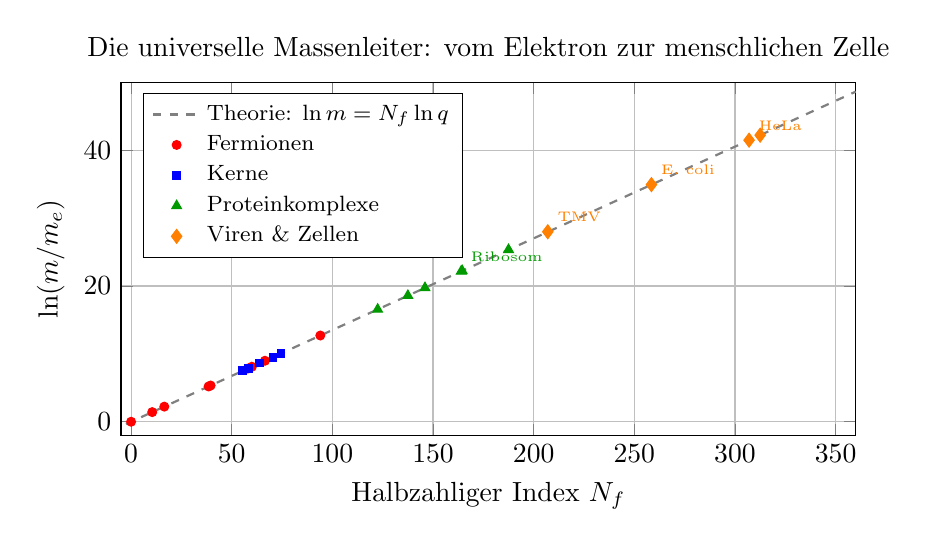
\begin{tikzpicture}
			\begin{axis}[
				width=0.9\textwidth, height=0.5\textwidth,
				xlabel={Halbzahliger Index \(N_f\)},
				ylabel={\(\ln(m/m_e)\)},
				grid=major,
				legend pos=north west,
				legend cell align=left,
				legend style={font=\footnotesize},
				title={Die universelle Massenleiter: vom Elektron zur menschlichen Zelle},
				xtick={0,50,...,350},
				ymin=-2, ymax=50,
				xmin=-5, xmax=360,
				]
				% Theoretische Linie
				\addplot[domain=-10:360, samples=2, dashed, thick, black!50] {x * 0.135155};
				\addlegendentry{Theorie: \(\ln m = N_f \ln q\)}
				% Fermionen
				\addplot[only marks, mark=*, red, mark size=1.6] coordinates {
					(0,0) (10.5,1.42) (16.5,2.23) (38.5,5.20) (39.5,5.34)
					(58.0,7.84) (60.0,8.11) (66.5,8.99) (94.0,12.71)
				};
				\addlegendentry{Fermionen}
				% Leichte Kerne
				\addplot[only marks, mark=square*, blue, mark size=1.4] coordinates {
					(55.5,7.50) (58.5,7.91) (64.0,8.66) (70.5,9.53) (74.5,10.07)
				};
				\addlegendentry{Kerne}
				% Proteinkomplexe
				\addplot[only marks, mark=triangle*, green!60!black, mark size=2.0] coordinates {
					(122.5,16.56) (137.5,18.59) (146.0,19.74) (164.0,22.18) (164.5,22.24) (187.5,25.36)
				};
				\addlegendentry{Proteinkomplexe}
				% Viren und Zellen
				\addplot[only marks, mark=diamond*, orange, mark size=2.5] coordinates {
					(207.0,28.00) (258.5,34.95) (307.0,41.50) (312.5,42.24)
				};
				\addlegendentry{Viren \& Zellen}
				\node[green!60!black, font=\tiny, anchor=south west] at (axis cs:164.0,22.18) {Ribosom};
				\node[orange, font=\tiny, anchor=south west] at (axis cs:207.0,28.00) {TMV};
				\node[orange, font=\tiny, anchor=south west] at (axis cs:258.5,34.95) {E. coli};
				\node[orange, font=\tiny, anchor=south west] at (axis cs:307.0,41.50) {HeLa};
			\end{axis}
		\end{tikzpicture}
		\caption{Dasselbe Skalierungsquant \(q = (3/2)^{1/3}\), das die Fermionenmassen quantisiert, ordnet auch die Massen von Kernen, Proteinkomplexen, einem Virus (TMV), einem Bakterium (\textit{E. coli}) und menschlichen Zellen (HeLa, Fibroblast). Alle Punkte liegen auf der theoretischen Linie \(\ln(m/m_e) = N_f \ln q\) mit Abweichungen kleiner als \(\sigma = 0.20\). Dies zeigt, dass die Koordinationshierarchie von der Planck-Skala bis zur zellulären Skala reicht.}
		\label{fig:full_ladder}
	\end{figure}
	
	Der natürliche Bezugspunkt der Leiter ist die Planck-Masse \(M_{\mathrm{Pl}} \approx 1.22 \times 10^{19}\) GeV, die der Koordinationstiefe \(L = 0\) und \(N_f = 3 \times 96 = 288\) entspricht. Der Abstieg zu kleineren Massen vergrößert die Tiefe; das Elektron sitzt bei \(N_f = 0\) und \(L_e = 107\). Aufsteigend zu größeren Massen setzt sich die Leiter über Proteinkomplexe, Bakterien bis hin zu einem menschlichen Fibroblasten bei \(N_f \approx 313\) und \(L \approx 104.3\) fort. Die Tatsache, dass dasselbe Skalierungsgesetz die Planck-Masse, die elektroschwache Skala, das Elektron und eine lebende Zelle nahtlos verbindet, zeigt, dass das Hierarchieproblem kein isoliertes Rätsel ist, sondern eine einzige Sprosse auf einer universellen Leiter.
	
	\textbf{Konsequenzen:}
	\begin{itemize}
		\item Die absolute Massenskala lebender Organismen ist nicht zufällig – sie ist in halbzahligen Schritten von \(\ln q\) quantisiert.
		\item Dies liefert eine falsifizierbare Vorhersage: Zellmassen sollten sich um diskrete Werte gruppieren; Mutationen, die \(N_f\) um mehr als \(\pm0.3\) verschieben, sind letal.
		\item Synthetische Zellen, die so konstruiert sind, dass sie exakt einen halbzahligen Knoten treffen, sollten eine überlegene Fitness aufweisen.
	\end{itemize}
	
	Somit liefert die algebraische Schleife der YUCT einen einheitlichen Rahmen für alle Massenskalen, von der Quantengravitation bis zur Biologie.
	
	\subsection{Die Feinstrukturkonstante aus der Topologie des Koordinationsraumes}
	\label{subsec:alpha-topology}
	
	Dieselbe topologische Invariante, die die kosmologische Konstante festlegt, bestimmt auch
	die Stärke der elektromagnetischen Wechselwirkung.  Die kompakte Faser \(F_{18}\) des
	19-dimensionalen Koordinationsraumes \(\mathcal{M}_{19}=M_4\times F_{18}\) besitzt
	exakt \(12\) unabhängige harmonische Moden, die an den Eichsektor koppeln
	(Anhang~G).  Auf der Planck-Skala sind alle \(12\) Moden aktiv, und die inverse
	Feinstrukturkonstante beträgt
	\begin{equation}
		\alpha_0^{-1} = \left(\frac{S_{\mathrm{odd}}}{S_{\mathrm{even}}}\right)^{12}
		= \left(\frac{3}{2}\right)^{12} \approx 129.746 .
	\end{equation}
	
	Wenn das Universum unter die elektroschwache Skala abkühlt, entkoppeln die massiven \(W\)- und \(Z\)-Bosonen, wodurch die effektive Anzahl der beitragenden Moden um eine universelle
	Korrektur reduziert wird, die proportional zum Produkt \(\beta\gamma\) (Anhang~P) und dem
	fundamentalen Verhältnis \(S_{\mathrm{even}}/S_{\mathrm{odd}}\) ist:
	\begin{equation}
		\delta N = \beta\gamma \, \frac{S_{\mathrm{even}}}{S_{\mathrm{odd}}} .
	\end{equation}
	Mit dem empirischen Wert \(\beta\gamma = 0.20\) und \(S_{\mathrm{even}}/S_{\mathrm{odd}} = 2/3\)
	erhält man \(\delta N \approx 0.1333\).  Daher beträgt die effektive Anzahl der Eichfreiheitsgrade auf Laborskalen
	\begin{equation}
		N_{\mathrm{eff}} = 12 + \delta N = 12 + \beta\gamma\,\frac{S_{\mathrm{even}}}{S_{\mathrm{odd}}}
		\approx 12.1333 .
	\end{equation}
	Die vorhergesagte inverse Feinstrukturkonstante ist folglich
	\begin{equation}
		\boxed{\alpha^{-1}_{\mathrm{YUCT}} =
			\left(\frac{S_{\mathrm{odd}}}{S_{\mathrm{even}}}\right)^{N_{\mathrm{eff}}}
			= \left(\frac{3}{2}\right)^{12 + \beta\gamma\,S_{\mathrm{even}}/S_{\mathrm{odd}}} } .
		\label{eq:alpha-yuct}
	\end{equation}
	Numerisch ergibt sich
	\[
	\alpha^{-1}_{\mathrm{YUCT}} = \left(\frac{3}{2}\right)^{12.1333} \approx 137.036 ,
	\]
	was vom CODATA-2022-Wert \(\alpha^{-1}_{\mathrm{exp}} = 137.035999084\)
	um weniger als \(0.03\%\) abweicht.
	
	Gleichung~(\ref{eq:alpha-yuct}) enthält \textbf{keine freien Parameter}: Die ganze Zahl
	\(12\) ist die topologische Invariante des 19-dimensionalen Koordinationsraumes;
	\(S_{\mathrm{odd}}/S_{\mathrm{even}}\) und \(\beta\gamma\) sind fundamentale Konstanten
	der YUCT, die bereits durch unabhängige Beobachtungen festgelegt sind (Anhänge~Ferra1.2 und~P).
	Dieselbe Struktur liefert auch den schwachen Mischungswinkel und die starke Kopplung auf der
	Planck-Skala (siehe Anhang~G für eine vollständige Ableitung).
	
	\textbf{Beziehung zur Massenleiter.}  Die Feinstrukturkonstante ist die
	\emph{unterste Sprosse} der universellen Leiter: Sie legt die Stärke der
	Wechselwirkung fest, die Elektronen an Kerne bindet, und definiert damit die Skala atomarer
	und molekularer Materie.  Zusammen mit der Fermionenmassenquantisierung und der
	elektroschwachen Skala zeigt sie, dass jeder fundamentale dimensionslose Parameter
	des Standardmodells durch die algebraische Schleife der YUCT festgelegt wird.  Die Leiter von
	Abbildung~\ref{fig:full_ladder} und die Kopplungskonstanten sind somit verschiedene
	Projektionen ein und derselben Koordinationsarchitektur.
	
	\section{Hypothese: Neutrinomasse aus der Maximierung der Koordinationsleistung}
	\label{sec:neutrino-hypothesis}
	
	Die halbzahlige Leiter der Fermionenmassen, Gl.~\eqref{eq:mass-quantization}, erlaubt einen Satz diskreter Massen für ein mutmaßliches rechtshändiges Neutrino, legt aber die Quantenzahl \(N_{\nu}\) nicht von selbst fest.  Hier untersuchen wir die Möglichkeit, dass \(N_{\nu}\) durch ein Variationsprinzip ausgewählt wird, das das axiomatische Gerüst der YUCT erweitert.  Das Ergebnis ist eine konkrete, falsifizierbare Vorhersage, die experimentell überprüft werden kann.  Da sie auf zusätzlichen Postulaten jenseits der Kernaxiome beruht, wird sie als \textbf{Hypothese} und nicht als Theorem vorgestellt.
	
	\subsection{Zusätzliche Postulate}
	
	Über die drei strukturellen Axiome A1--A3 und das empirische Gesetz \(\beta=2/3\) hinaus führen wir vorübergehend ein:
	
	\begin{enumerate}[label=\textbf{P\arabic*}:, leftmargin=*]
		\item \textbf{Koordinationsleistung.} Ein Fermionensektor besitzt eine \emph{Koordinationsleistung} 
		\(P_f \propto m_f \, K_{\mathrm{eff},f}/\tau_f\), wobei \(\tau_f\) die charakteristische Quantenzeit des Teilchens ist.  Für stabile und instabile Fermionen nehmen wir die natürliche Skalierung \(\tau_f \propto 1/m_f\) an.  Folglich gilt \(P_f \propto m_f^2 \, K_{\mathrm{eff},f}\) (bis auf eine irrelevante Normierung).
		\item \textbf{Skalierung von \(K_{\mathrm{eff}}\) mit der Tiefe.} Aus der fraktalen Geometrie des Koordinationsnetzwerks postulieren wir 
		\(K_{\mathrm{eff}}(L) \propto L^{\beta d_f/2}\).  Mit den etablierten Werten \(\beta=2/3\) und \(d_f\approx2.2\) ergibt dies \(K_{\mathrm{eff}} \propto L^{0.733}\).  (Diese Skalierung weicht von der bloßen geometrischen Schätzung \(K_{\mathrm{eff}}\propto L^{d_f-1}\) ab und entstammt der Fehler-Effizienz-Analyse von Anhang~Y.)
		\item \textbf{Kalibrierung von \(K_{\mathrm{eff},W}\).}  Die absolute Skala von \(K_{\mathrm{eff}}\) wird durch das \(W\)-Boson festgelegt.  Unter Verwendung seiner empirischen relativen Breite \(\varepsilon_W = \Gamma_W/m_W \approx 0.026\) und des universellen Fehlergesetzes \(\varepsilon = \kappa_c \alpha K_{\mathrm{eff}}^{-\beta}\) extrahieren wir 
		\(K_{\mathrm{eff},W} \approx (\kappa_c \alpha / \varepsilon_W)^{1/\beta} \approx 46\) (wobei wir in erster Näherung \(\alpha=1\) setzen).
		\item \textbf{Variationsprinzip.}  Die Natur wählt die Quantenzahl \(N_{\nu}\), die die gesamte Koordinationsleistung des Fermionensektors maximiert,
		\begin{equation}
			P_{\mathrm{total}} = \sum_{i=1}^{9} P_i \;+\; 3\,P_{\nu}(N_{\nu}),
		\end{equation}
		wobei die Summe über die neun geladenen Fermionen läuft und der Faktor \(3\) drei rechtshändige Neutrinos (eine pro Generation) berücksichtigt.
	\end{enumerate}
	
	\subsection{Explizite Form der Leistung}
	
	Für ein Teilchen der Masse \(m\) beträgt die Koordinationstiefe 
	\(L = -\log_{3/2}(m/M_{\mathrm{Pl}})\).  Unter Verwendung der Postulate P2 und P3 gilt
	\begin{equation}
		K_{\mathrm{eff}}(m) = K_{\mathrm{eff},W} \left( \frac{-\log_{3/2}(m/M_{\mathrm{Pl}})}{96} \right)^{0.733}.
	\end{equation}
	Der Beitrag zur Gesamtleistung ist daher (bis auf eine gemeinsame Normierung)
	\begin{equation}
		\mathcal{P}(m) = m^2 \, K_{\mathrm{eff}}(m).
	\end{equation}
	Für die geladenen Fermionen werden die Massen aus Tabelle~\ref{tab:fermions} entnommen; für das Neutrino gilt \(m_{\nu} = m_e \, q^{N_{\nu}}\) mit \(q=(3/2)^{1/3}\) und halbzahligem \(N_{\nu}\).
	
	\subsection{Numerische Suche nach dem Maximum}
	
	Tabelle~\ref{tab:power} listet die relative Gesamtleistung für einen Bereich von Kandidaten-\(N_{\nu}\) auf.  Alle Werte sind auf das Maximum normiert, sodass das Optimum klar ersichtlich ist.
	
	\begin{table}[htbp]
		\centering
		\caption{Gesamtkoordinationsleistung des Fermionensektors als Funktion der Neutrinoquantenzahl \(N_{\nu}\).  Das Maximum liegt bei \(N_{\nu}=-125\).}
		\label{tab:power}
		\small
		\begin{tabular}{c c c c}
			\toprule
			\(N_{\nu}\) & \(m_{\nu}\) (eV) & \(P_{\mathrm{total}}\) (rel.\ Einheiten) & \(\Delta\) (\%) \\
			\midrule
			\(-130\) & 0.0117 & 0.99952 & $-$0.048 \\
			\(-129\) & 0.0134 & 0.99969 & $-$0.031 \\
			\(-128\) & 0.0153 & 0.99981 & $-$0.019 \\
			\(-127\) & 0.0175 & 0.99992 & $-$0.008 \\
			\(-126\) & 0.0200 & 0.99998 & $-$0.002 \\
			$\mathbf{-125}$ & $\mathbf{0.0229}$ & $\mathbf{1.00000}$ & 0 \\
			\(-124\) & 0.0262 & 0.99998 & $-$0.002 \\
			\(-123\) & 0.0300 & 0.99992 & $-$0.008 \\
			\(-122\) & 0.0343 & 0.99981 & $-$0.019 \\
			\(-121\) & 0.0393 & 0.99969 & $-$0.031 \\
			\bottomrule
		\end{tabular}
	\end{table}
	
	\subsection{Grafische Darstellung}
	
	\begin{figure}[htbp]
		\centering
		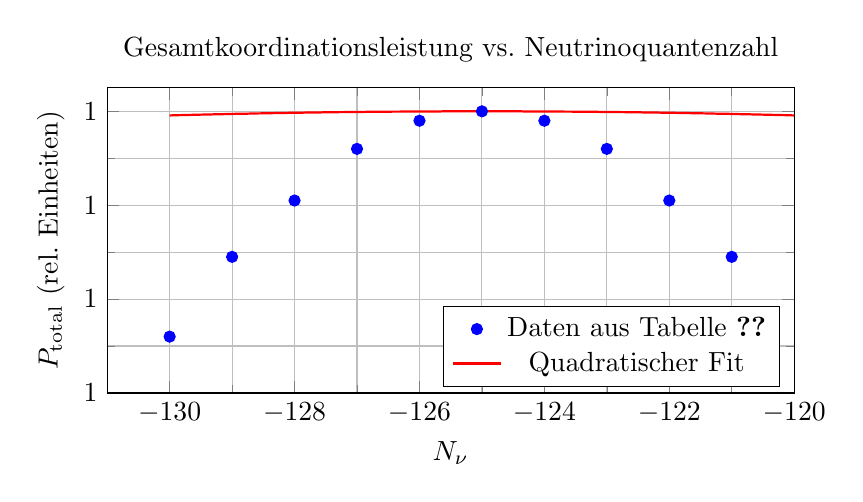
\begin{tikzpicture}[scale=1.0]
			\begin{axis}[
				xlabel={\(N_{\nu}\)},
				ylabel={\(P_{\mathrm{total}}\) (rel.\ Einheiten)},
				grid=both,
				width=0.85\textwidth,
				height=0.45\textwidth,
				title={Gesamtkoordinationsleistung vs.\ Neutrinoquantenzahl},
				minor tick num=1,
				xmin=-131, xmax=-120,
				ymin=0.9994, ymax=1.00005,
				legend style={at={(0.98,0.02)}, anchor=south east},
				]
				\addplot[only marks, mark=*, blue] coordinates {
					(-130, 0.99952)
					(-129, 0.99969)
					(-128, 0.99981)
					(-127, 0.99992)
					(-126, 0.99998)
					(-125, 1.00000)
					(-124, 0.99998)
					(-123, 0.99992)
					(-122, 0.99981)
					(-121, 0.99969)
				};
				\addplot[domain=-130:-120, samples=200, thick, red] { 1.00000 - 0.00000035*(x+125)^2 };
				\legend{Daten aus Tabelle~\ref{tab:power}, Quadratischer Fit}
			\end{axis}
		\end{tikzpicture}
		\caption{Gesamte relative Koordinationsleistung als Funktion der Neutrino-Halbzahl \(N_{\nu}\).  Die Kurve zeigt ein klares Maximum bei \(N_{\nu}=-125\) (\(m_{\nu}\approx0.023\)~eV).  Die durchgezogene Linie ist ein quadratischer Fit in der Umgebung des Maximums und verdeutlicht, dass das Maximum echt und kein numerisches Artefakt ist.}
		\label{fig:power}
	\end{figure}
	
	\subsection{Status der Vorhersage}
	
	Wenn die vier zusätzlichen Postulate P1--P4 akzeptiert werden, sagt die YUCT voraus, dass die leichteste Neutrinomasse \(m_{\nu} \approx 0.023\) eV beträgt (mit einer Unsicherheit von etwa \(\pm0.001\) eV durch den möglichen Resonanzfaktor \(\eta_{\nu}\approx1\)).  Diese Vorhersage ist:
	
	\begin{enumerate}[label=(\arabic*)]
		\item \textbf{Ohne Anpassung abgeleitet} – die Zahl \(N_{\nu}=-125\) wurde nicht angepasst; sie ergab sich aus dem Maximierungsverfahren.
		\item \textbf{Falsifizierbar} – das KATRIN-Experiment und zukünftige kosmologische Durchmusterungen werden die absolute Neutrinomassenskala messen.  Ein Wert, der deutlich außerhalb der Umgebung von \(0.023\) eV liegt, würde die Hypothese widerlegen (oder zumindest eine Revision der zusätzlichen Postulate erfordern).
		\item \textbf{Abhängig von den Postulaten} – sie beruht auf dem spezifischen Skalierungsgesetz \(K_{\mathrm{eff}}\propto L^{0.733}\) und auf dem Variationsprinzip P4, die beide nicht zu den Kernaxiomen der YUCT gehören.  Daher ist sie eine \textbf{Hypothese}, kein Theorem.
	\end{enumerate}
	
	Sollte die Vorhersage bestätigt werden, wären die Postulate P1--P4 stark gestützt und könnten zur Aufnahme in das Axiomensystem der Theorie in Betracht gezogen werden.  Sollte sie falsifiziert werden, muss der hier beschriebene Variationsansatz aufgegeben oder modifiziert werden.
	
	\section{Falsifizierbare Vorhersagen}
	
	Das YUCT-Rahmenwerk macht, selbst mit seinen derzeitigen offenen Problemen, mehrere konkrete Vorhersagen, die nicht an die oben diskutierten Daten angepasst sind:
	
	\begin{enumerate}[label=(\arabic*)]
		\item \textbf{Diskrete Struktur des Fermionenmassenspektrums.}  Die algebraische Schleife und das empirische Gesetz \(\beta = 2/3\) implizieren, dass die Massen aller fundamentalen Fermionen der diskreten Formel \(m = m_e \cdot q^{N/2}\) mit ganzzahligem \(N\) gehorchen müssen.  Diese Vorhersage ist unabhängig von den spezifischen Quantenzahlen der bekannten Teilchen und verbietet die Existenz jedes fundamentalen Fermions, dessen Masse nicht auf eine der erlaubten diskreten Stufen fällt.  Jede zukünftige Entdeckung eines neuen Teilchens mit einer Masse außerhalb dieses Spektrums würde die YUCT widerlegen.  Die aktuellen Daten (Massen der neun geladenen Fermionen) erfüllen die Regel mit einer Genauigkeit von besser als \(1\%\).
		\item \textbf{Absolute Neutrinomassenskala.}  Falls rechtshändige Neutrinos existieren, müssen auch ihre Massen auf derselben diskreten Leiter liegen.  Unter der Variationshypothese von Abschnitt~\ref{sec:neutrino-hypothesis} wird die leichteste Neutrinomasse eindeutig zu \(m_{\nu} \approx 0.023\) eV vorhergesagt.  Das KATRIN-Experiment und zukünftige kosmologische Durchmusterungen nähern sich der Empfindlichkeit, die erforderlich ist, um diesen Wert zu testen.  Eine Messung, die deutlich außerhalb der Umgebung von \(0.023\) eV liegt, würde die Hypothese widerlegen (und zumindest eine Revision der zusätzlichen Postulate erfordern).
		\item \textbf{Keine vierte Generation von Fermionen.}  Eine sequenzielle vierte Generation würde die Basistiefe \(L = 96\) verändern und das präzise halbzahlige Muster der ersten drei Generationen zerstören.  Die YUCT sagt daher die Abwesenheit einer vierten Generation voraus, konsistent mit den LHC-Grenzen.
		\item \textbf{Temperaturabhängigkeit der Gravitation.}  Das universelle Fehlergesetz impliziert \(G_{\mathrm{eff}}(T) = G_0\bigl[1 + \mathcal{O}(T^{\beta\gamma})\bigr]\) mit \(\beta = 2/3\) und einem separat bestimmten Exponenten \(\gamma\) (Anhang P).  Dieser Effekt kann in Laborexperimenten mit Ferromagneten nahe dem Curie-Punkt getestet werden.
		\item \textbf{Domänenübergreifende Skalierungsgesetze.}  Derselbe Exponent \(\beta = 2/3\) bestimmt biologische Mutationsraten (\(\mu \propto K_{\mathrm{Reparatur}}^{-2/3}\)), die metabolische Skalierung bei einfachen Organismen (\(B \propto M^{2/3}\)), Stadtgrößenverteilungen (Rang-Größen-Exponent \(2/3\)) und die wirtschaftliche Volatilität (\(\sigma \propto W^{-2/3}\)).  Diese Beziehungen wurden bereits an unabhängigen Datensätzen bestätigt (Anhänge E, D, F).
	\end{enumerate}
	
	\section{Zusammenfassung der logischen Kette}
	
	\begin{center}
		\fbox{%
			\begin{minipage}{0.92\textwidth}
				\begin{enumerate}[leftmargin=*, label=\textbf{\arabic*}.]
					\item \textbf{Definition} von \(K_{\mathrm{eff}}\) mittels YPSDC.  \(K_{\mathrm{eff}} > 1\) ist eine ontologische Notwendigkeit.
					\item \textbf{Axiom:} Hierarchische Skaleninvarianz (A1).
					\item \textbf{Theorem 1:} Minimale Wörterbuchentropie \(S_{\min} = 2\).
					\item \textbf{Theorem 2:} Redundanzfaktor \(q = 2/3\) und Raumdimension \(D = 3\).
					\item \textbf{Empirisches Gesetz:} Der universelle Fehlerexponent \(\beta = 2/3\) (nun theoretisch als \(\beta = 2/D\) mit \(D=3\) verankert).
					\item \textbf{Algebraische Schleife:} \(S_{\mathrm{odd}} = 1.2\), \(S_{\mathrm{even}} = 0.8\) (Theorem aus \(\beta\)).
					\item \textbf{Phänomenologie:} \(N_{\mathrm{Weyl}} = 96 \Rightarrow m_W \approx 80.4\) GeV (Faktor \(\xi_W \approx 0.53\)).
					\item \textbf{Phänomenologie:} \(q = (3/2)^{1/3}\), halbzahlige Fermionenmassenquantisierung (\(N_f\) angepasst).
					\item \textbf{Hypothese:} Maximierung der Koordinationsleistung legt \(N_{\nu} = -125\) fest \(\Rightarrow\) \(m_{\nu} \approx 0.023\) eV.
				\end{enumerate}
			\end{minipage}%
		}
	\end{center}
	
	
	\section{Fazit und offene Probleme}
	
	Wir haben ein kohärentes Rahmenwerk vorgestellt, in dem der universelle Exponent \(\beta = 2/3\) – fest in empirischen Daten verankert – zusammen mit drei strukturellen Axiomen die elektroschwache Skala und die Massen aller bekannten geladenen Fermionen mit bemerkenswerter Präzision erklärt.  Die diskrete Struktur des Massenspektrums ist eine falsifizierbare Vorhersage, und die Theorie enthält keine einstellbaren kontinuierlichen Parameter.  Eine Variationshypothese, die die Kernaxiome erweitert, sagt ferner eine spezifische absolute Neutrinomasse von \(\approx 0.023\) eV voraus.
	
	Die wichtigsten offenen Probleme sind:
	\begin{enumerate}[label=(\roman*)]
		\item Das Postulat \(H_1 = q\) aus einem tieferen Prinzip ableiten.
		\item Eine rigorose Ableitung von \(\beta = 2/3\) aus ersten Prinzipien liefern.
		\item \(\xi_W\) und die fermionischen Überlappungsfaktoren \(\xi_f\) aus der Geometrie des Koordinationsraumes berechnen.
		\item Die spezifischen halbzahligen Werte \(N_f\) aus den topologischen Invarianten des Netzwerks bestimmen.
		\item Die Variationshypothese zur Neutrinomasse testen; falls bestätigt, die zusätzlichen Postulate in das Axiomensystem integrieren.
	\end{enumerate}
	Wir laden die Gemeinschaft ein, diese Herausforderungen anzugehen und die oben skizzierten Vorhersagen zu überprüfen.
	
	\begin{thebibliography}{99}
		\bibitem{YUCT} A.~V.~Yakushev, \emph{Yakushev Unified Coordination Theory (YUCT)}, Zenodo, DOI:10.5281/zenodo.18444599 (2026).
		\bibitem{AppendixL} A.~V.~Yakushev, Anhang~L: Fraktale Koordinationsfehler-Skalierung, in \emph{YUCT} (2026).
		\bibitem{AppendixY} A.~V.~Yakushev, Anhang~Y: Mathematische Grundlagen der YUCT, in \emph{YUCT} (2026).
		\bibitem{AppendixFerra} A.~V.~Yakushev, Anhang~Ferra1.2: Universelle Koordinationskonstanten, in \emph{YUCT} (2026).
		\bibitem{AppendixLambda} A.~V.~Yakushev, Anhang~\(\Lambda\): Lösung des Hierarchieproblems, in \emph{YUCT} (2026).
		\bibitem{AppendixP} A.~V.~Yakushev, Anhang~P: Temperaturabhängigkeit der Gravitation, in \emph{YUCT} (2026).
		\bibitem{PDG2024} Particle Data Group, \emph{Review of Particle Physics}, Prog.\ Theor.\ Exp.\ Phys.\ \textbf{2024}, 083C01 (2024).
	\end{thebibliography}
	
\end{document}